\begin{pastexam}[label={px:ccu-114-swa-06}]{中正資工所甲組 114 學年度 第 6 題}
（複選）

(5\%) (Select \underline{multiple} correct answers) Which of the following statements is (are) true?

\begin{center}
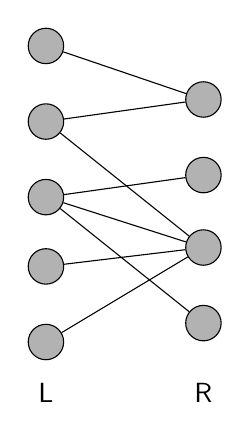
\begin{tikzpicture}[v/.style={circle,draw,fill=gray!60,minimum size=4.5mm,inner sep=0pt},scale=0.8]
\foreach \i/\y in {1/0.8,2/2.0,3/3.2,4/4.3,5/5.5} \node[v] (L\i) at (0,-\y) {};
\foreach \i/\y in {1/1.65,2/2.85,3/4.0,4/5.2} \node[v] (R\i) at (2.5,-\y) {};
\foreach \a/\b in {L1/R1,L2/R1,L2/R3,L3/R2,L3/R3,L3/R4,L4/R3,L5/R3} \draw (\a)--(\b);
\node at (0,-6.3) {\textsf{L}}; \node at (2.5,-6.3) {\textsf{R}};
\end{tikzpicture}
\end{center}
\begin{enumerate}[label=(\alph*)]
\item Given a dense graph with negative weight edges but no negative weight cycles, applying Johnson's
algorithm on this graph will be faster than running Floyd-Warshall algorithm.
\item The class NP contains problems that are solvable in polynomial time.
\item The halting problem is NP-hard problem.
\item Ford-Fulkerson method can be used to find a maximum matching from the graph at the right side
\item Following (d), the graph has maximal cardinality 4.
\end{enumerate}
\end{pastexam}

\begin{pastsoln}
答案：(b)(c)(d)。

本題的 (a) 屬資結書第~25~章，(b)(c) 屬第~28~章，(d)(e) 屬第~26~章（二分匹配）。 原卷的圖在選項右邊，
這裡排在選項上面。 圖的左邊由上而下記為 $L_1, \ldots, L_5$，右邊記為 $R_1, \ldots, R_4$，邊是
$L_1R_1$、$L_2R_1$、$L_2R_3$、$L_3R_2$、$L_3R_3$、$L_3R_4$、$L_4R_3$、$L_5R_3$。

\begin{itemize}
\item (a) 錯。 Johnson 演算法先用 Bellman--Ford 重新加權（$O(VE)$），再從每個頂點跑一次 Dijkstra；用
費氏堆積時總時間 $O(V^2 \log V + VE)$（資結書第~25.7~節）。 稠密的圖 $E = \Theta(V^2)$，這是
$\Theta(V^3)$，和 Floyd--Warshall 的 $\Theta(V^3)$ 同階，不會比較快；用二元堆積的 Dijkstra 更是
$O(VE \log V) = O(V^3 \log V)$，反而比較慢。 Johnson 的優勢在稀疏的圖。
\item (b) 對。 多項式時間解得出來的問題（P），也能在多項式時間驗證（驗證時不理會證據，直接解一次），
所以 $\mathrm{P} \subseteq \mathrm{NP}$（資結書第~28.2~節）。
\item (c) 對。 停機問題是 NP 難的：任何 NP 問題都能歸約到它（資結書第~28.4~節的例子，例如把
\textsf{SAT} 的公式 $\phi$ 轉成「一個程式：窮舉所有指派，找到滿足的就停，否則進入無窮迴圈」，程式會停
若且唯若 $\phi$ 可滿足）。 它不可判定，所以不在 NP 裡，不是 NP 完備，但是 NP 難。
\item (d) 對。 加一個源點 $s$ 連到每個 $L_i$、每個 $R_j$ 連到匯點 $t$，原來的邊由 $L$ 指向 $R$，容量
全部是 $1$；整數的最大流就對應最大匹配（資結書第~26.6.2~節），用 Ford--Fulkerson 求最大流即可。
\item (e) 錯。 最大匹配只有 $3$ 條邊。 $R_2$ 和 $R_4$ 都只和 $L_3$ 相連，$L_3$ 只能配一個，所以 $R_2$、
$R_4$ 最多配到一個；$R_1$、$R_3$ 各最多一個。 匹配最多 $3$ 條，例如 $\{L_1R_1, L_2R_3, L_3R_2\}$
就有 $3$ 條。 用最大流驗證，增廣三次後剩餘網路裡 $s$ 走不到 $t$，最大流是 $3$。 所以不是 $4$。
\end{itemize}
\end{pastsoln}
